\newpage
\section{Speech Signal Processing}

\subsection{Analog-to-Digital Conversion}
Voices in real life are analog signals, hence before conducting digital signal processing techniques, analog-to-digital conversions are required.\\

Given a continuous-time signal $s(t)$, we define the \textit{sampled signal} by
\begin{equation}
s[n] = s(nT_s) = s(\frac{n}{F_s})
\end{equation}
where $T_s$ is the sampling interval and $F_s$ is the sampling rate.\\

$T_s$ should be carefully chosen in order to avoid distortion caused by aliasing. Telephony since the 1950s limits the information bandwidth to 300-3400 Hz \cite{EVW-report}. However, in normal conversational speech, the frequency content is mainly between 0-8000 Hz \cite{uysal2005bandwidth}. According to Nyquist-Shannon sampling theorem, we set the folding frequency $\frac{F_s}{2}$ = 8000 Hz, i.e. $F_s$ = 16 kHz.

%--------------------------------------------
%--------------------------------------------

\subsection{Pre-emphasis}

%--------------------------------------------
%--------------------------------------------

\subsection{Framing \& Windowing}

%--------------------------------------------
%--------------------------------------------

\subsection{Threshold}

%--------------------------------------------
%--------------------------------------------

\subsection{Mel Filter Bank Processing}

\subsubsection{Power Spectrum}

%--------------------------------------------

\subsubsection{Bank Filtering}

\begin{figure}[H]
\centering
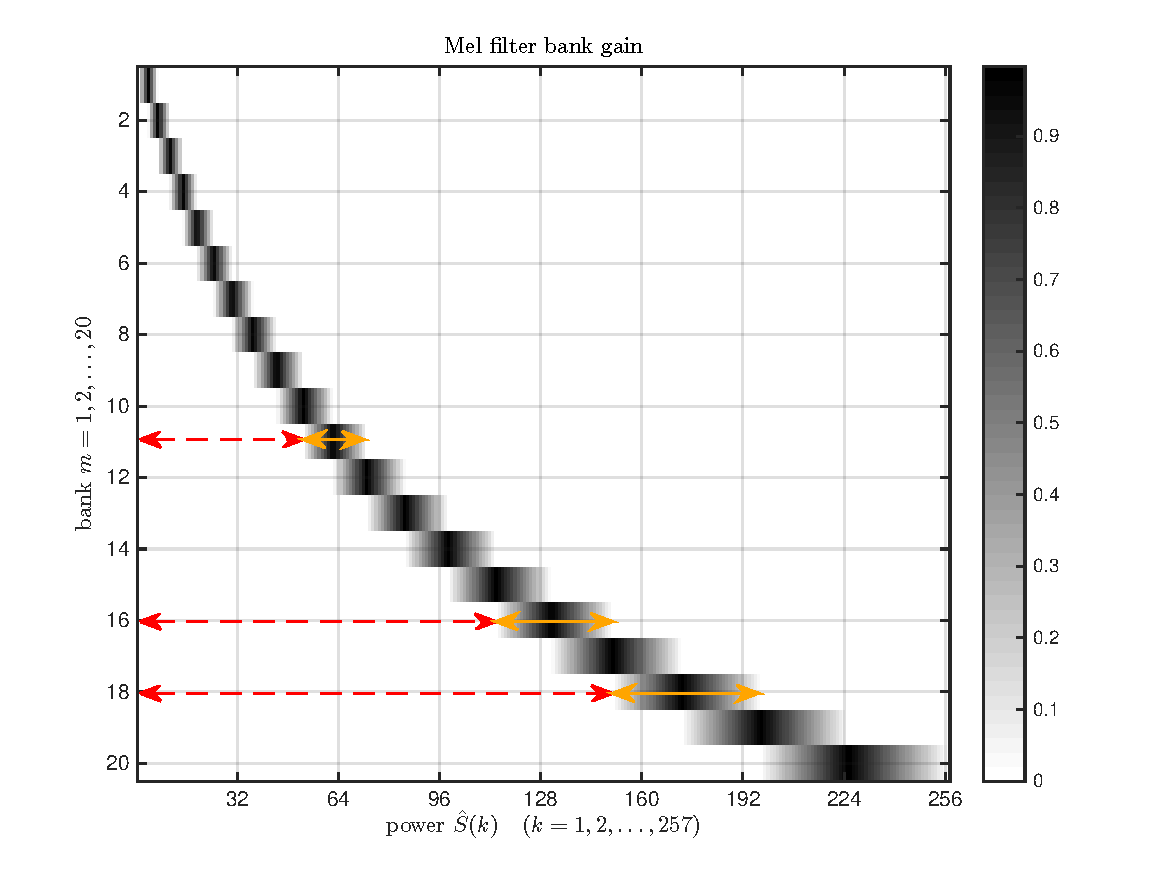
\includegraphics[width=6in]{ang/mel_filter_bank_gain}
\caption{Mel Filter Bank Gain}
\end{figure}

\begin{figure}[H]
\centering
\includegraphics[width=6in]{ang/mel_bank_9}
\caption{Bank Filtering Demonstration}
\end{figure}

%--------------------------------------------

\subsubsection{Log Scaling}

%--------------------------------------------

\subsubsection{Discrete Cosine Transform}
